The UST algorithm as described in \cite{bib11} formulates style transfer as an image reconstruction process coupled with feature transformation of whitening and coloring (WCT). The reconstruction step is responsible for inverting features back to the RGB space, the feature transformation step matches the feature statistics of a content image to a style image. The file \texttt{universal\_style\_transfer.py} implements the UST algorithm, use '\texttt{python universal\_style\_transfer.py -h}' for help.

\subsubsection{Architecture}\label{subsec:arch}
The basic building block of the UST is a pair of VGG based encoder and decoder, explained and described in section ~\ref{models_methods_lbl}. A single level stylization pass in UST would be to pass a content image and a style image through an encoder, perform a transformation called WCT on the extracted content features, and then to reconstruct the output of the WCT using the decoder. The image output by the decoder should have both the original content and some notion of the artistic styles in the style image. To achieve better results, UST does more than a single level stylization pass, it constructs a pipeline of such levels, each with its own encoder-decoder pair. Passing the content through this pipeline transfers style in different feature depths, so the result is generally more pleasing. See figure ~\ref{fig:full-pipeline} for a block diagram of the pipeline pass to perform UST on a pair of images $c,s$. In the following sections, for the $j$-th level of the pipeline denote the encoder by $E_j$ and the decoder by $D_j$.

\begin{figure}[h!]
	\centering
	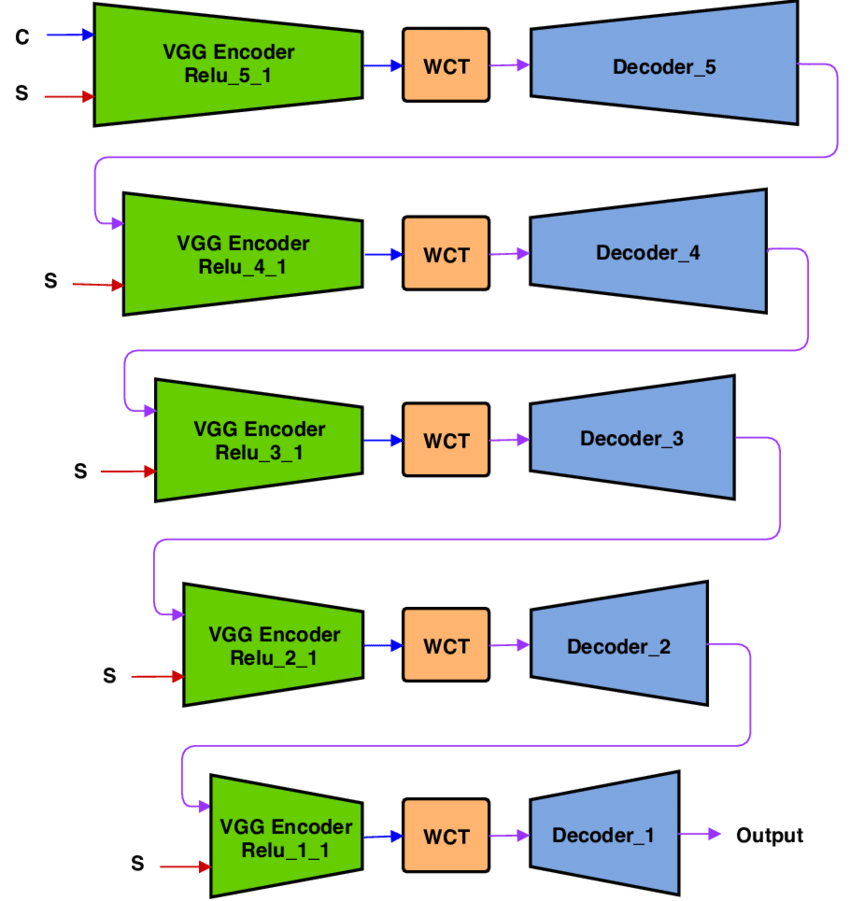
\includegraphics[width=0.5\linewidth]{UST_arc_mlt_level_pipeline.png}
	\caption{Universal Style Transfer pipeline architecture. Each level of stylization consists of single encoder-WCT-decoder network with different decreasing number of VGG layers. C and S are content and style images, respectively.
	}
	\label{fig:full-pipeline}
\end{figure}

\subsubsection{WCT} As explained above, given a pair of content image $I_C$ and style image $I_S$ as input for the $j$-th level, at first the encoder extracts their features by $f_c = E_j(I_C)$, $f_s = E_j(I_S)$. Notice that these features are three dimensional, $f_c$ is $[c\times h \times w]$ and $f_s$ is $[c\times h' \times w']$. Their height and width are generally different but their number of channels, $c$, is the same. The WCT is a pair of projection functions working on vectorized VGG features. The term \textit{vectorized} means that we treat every channel of the feature tensor as a row vector, so $\vec{f_c}$ is $[c \times hw]$ and $\vec{f_s}$ is $[c \times h'w']$. WCT works on the features extracted by the encoder, and its result is fed to the decoder, as seen in Figure ~\ref{fig:full-pipeline}. WCT is a composition of a whitening transform ($\hat{f}_C$) and a coloring transform ($\hat{f}_{CS}$). The key idea behind the WCT is to directly match feature correlations of the content image to those of the style image via those two projections. Specifically, the WCT transform is applied to the vectorized content and style feature $\vec{f_c}$, $\vec{f_s}$ respectively via:\\

%%%%%%%%%%%%%%%%%%whitening%%%%%%%%%%%%%%%%%%%%%%
\textbf{Whitening:}\\
\begin{equation}
Centered\_\vec{f_c} = \vec{f_c} - mean(\vec{f_c})
\end{equation}
\begin{equation}
\hat{f_c}\hat{f_c}^T=I \Rightarrow  \hat{f_c} = E_cD_c^{-\frac{1}{2}}E_c^T \cdot Centered\_\vec{f_c} 
\end{equation}
Where $D_c$ is a diagonal matrix with the eigenvalues of the covariance matrix:
\begin{equation*}
Centered\_\vec{f_c} \cdot Centered\_\vec{f_c}^T=E_c D_c E_c^T \in\mathbb{R}^{cxc}
\end{equation*}
and $E_c$ is the corresponding orthogonal matrix of eigenvectors, (see figure ~\ref{fig:WCT-vis} (a)). Both matrices obtained by using Singular Value Decomposition (SVD).\\

%%%%%%%%%%%%%%%%%%coloring%%%%%%%%%%%%%%%%%%%%%%
\textbf{Coloring:}\\
Coloring transform is the inverse of the whitening transform, see figure ~\ref{fig:WCT-vis} (b)).
\begin{equation}
Centered\_\vec{f_s} = \vec{f_s} - mean(\vec{f_s})
\end{equation}
\begin{equation}
\hat{f_{cs}}\hat{f_{cs}}^T=f_sf_s^T \Rightarrow  \hat{f_{cs}} = E_sD_s^{\frac{1}{2}}E_s^T\hat{f_c} 
\end{equation}
Where $D_s$ is a diagonal matrix with the eigenvalues of the covariance matrix:  \begin{equation*}
Centered\_\vec{f_s}\cdot Centered\_\vec{f_s}^T \in\mathbb{R}^{cxc}
\end{equation*}
and $E_s$ is the corresponding orthogonal matrix of eigenvectors, both matrices also obtained by SVD. Finally, add the mean vector of the style:
\begin{equation}
\hat{f_{cs}} = \hat{f_{cs}}+mean(\vec{f_s})
\end{equation}

After the transformation, the correlations of transformed content features match those of the style, i.e., $\hat{f_{cs}} \hat{f_{cs}}^T = \vec{f_s} \vec{f_s}^T$.
The WCT performs well for artistic image stylization. However it generates
structural artifacts (e.g., distortions on object boundaries)
WCT is implemented in the function \texttt{wct} in file \texttt{utils.py}.

\begin{figure}[h!]
	\centering
	\begin{subfigure}[b]{0.4\linewidth}
		\includegraphics[width=\linewidth]{whitening.png}
		\caption{Data whitening}
	\end{subfigure}
	\begin{subfigure}[b]{0.4\linewidth}
		\includegraphics[width=\linewidth]{coloring.png}
		\caption{Data coloring}
	\end{subfigure}
	\caption{Whitening-Coloring-Transformation}
	\label{fig:WCT-vis}
\end{figure}

\subsubsection{Texture Synthesis}\label{subsec:texture}
UST has application as universal texture synthesizer too. To conduct texture synthesis, simply perform UST while setting the content image as a random noise image. The evaluation criterion for the quality of the synthesized texture is usually human inspection and textures are successfully synthesized if a human observer cannot tell the original texture from a synthesized one.

\subsubsection{CLI Tool}
Our Implementation of UST is meant to serve as a CLI tool both useful to users and researchers. Its functionalities include style transfer, merge-style transfer, texture synthesis. It also supports the $\alpha$ and $\beta$ parameters as described in \cite{bib11}. All these are important for users. For researchers and developers our implementation should appeal as well, mainly thanks to two special features:
\begin{enumerate}
	\item Custom stylization pipeline architecture. The argument \texttt{--arch} is ready to receive any 1-5 digit sequence to build a specific tailored pipeline architecture. The default is "54321". Using this, researchers can study different architectures and their effect on style transfer.
	\item The \texttt{ref\_models\_factory.py} is an interface for using custom encoder-decoder networks. Researchers and developers can easily implement their own \texttt{ref\_models\_factory.py} file to test the effectiveness of their models in the style transfer task.
\end{enumerate} 